\documentclass{article}
\usepackage{tikz}
\usetikzlibrary{arrows.meta,positioning,calc,shapes.geometric}
\pagestyle{empty}
\begin{document}
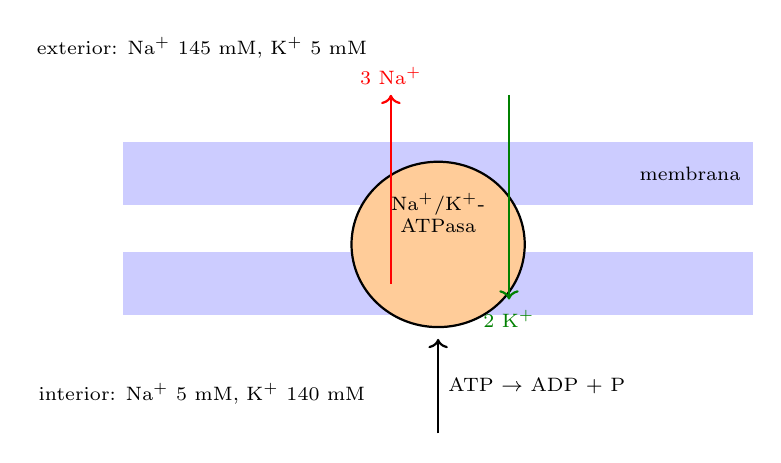
\begin{tikzpicture}
\tikzset{every node/.append style={align=center}}

\fill[blue!20] (0,1.0) rectangle (8,1.8); \fill[blue!20] (0,-0.4) rectangle (8,0.4); \node[font=\scriptsize] at (7.2,1.4) {membrana}; 
\draw[fill=orange!40, thick] (4,0.5) ellipse (1.1 and 1.05); \node[font=\scriptsize, align=center] at (4,0.9) {Na$^+$/K$^+$-\\ATPasa};
\node[font=\scriptsize] at (1,3.0) {exterior: Na$^+$ 145 mM, K$^+$ 5 mM}; \node[font=\scriptsize] at (1,-1.4) {interior: Na$^+$ 5 mM, K$^+$ 140 mM};
\draw[->, thick, red] (3.4,0.0) -- (3.4,2.4) node[above, font=\scriptsize] {3 Na$^+$};
\draw[->, thick, green!50!black] (4.9,2.4) -- (4.9,-0.2) node[below, font=\scriptsize] {2 K$^+$};
\draw[->, thick] (4,-1.9) -- (4,-0.7) node[midway, right, font=\scriptsize] {ATP $\to$ ADP + P};

\end{tikzpicture}
\end{document}
